\begin{frame}{Wodurch und wie entstehen Gamma Ray Bursts?}
  \begin{columns}
 \begin{column}{0.4\textwidth}
  \begin{itemize}
    \item  Man weiß es nicht
    \item  Bei manchen Gamma Ray Bursts: Supernova
  \end{itemize}
\vspace{2em}
\end{column}
\begin{column}{0.6\textwidth}
  evtl hier noch ein Bild

\end{column}
  \end{columns}
\end{frame}




\begin{frame}{Liegt es an der Zusammensetzung der Erdatmosphäre, dass nicht alle Frequenzen durchgelassen werden? Und wie kommt es, dass bestimmte Frequenzbereiche nicht durchgelassen werden?}
  \begin{figure}
    \centering
    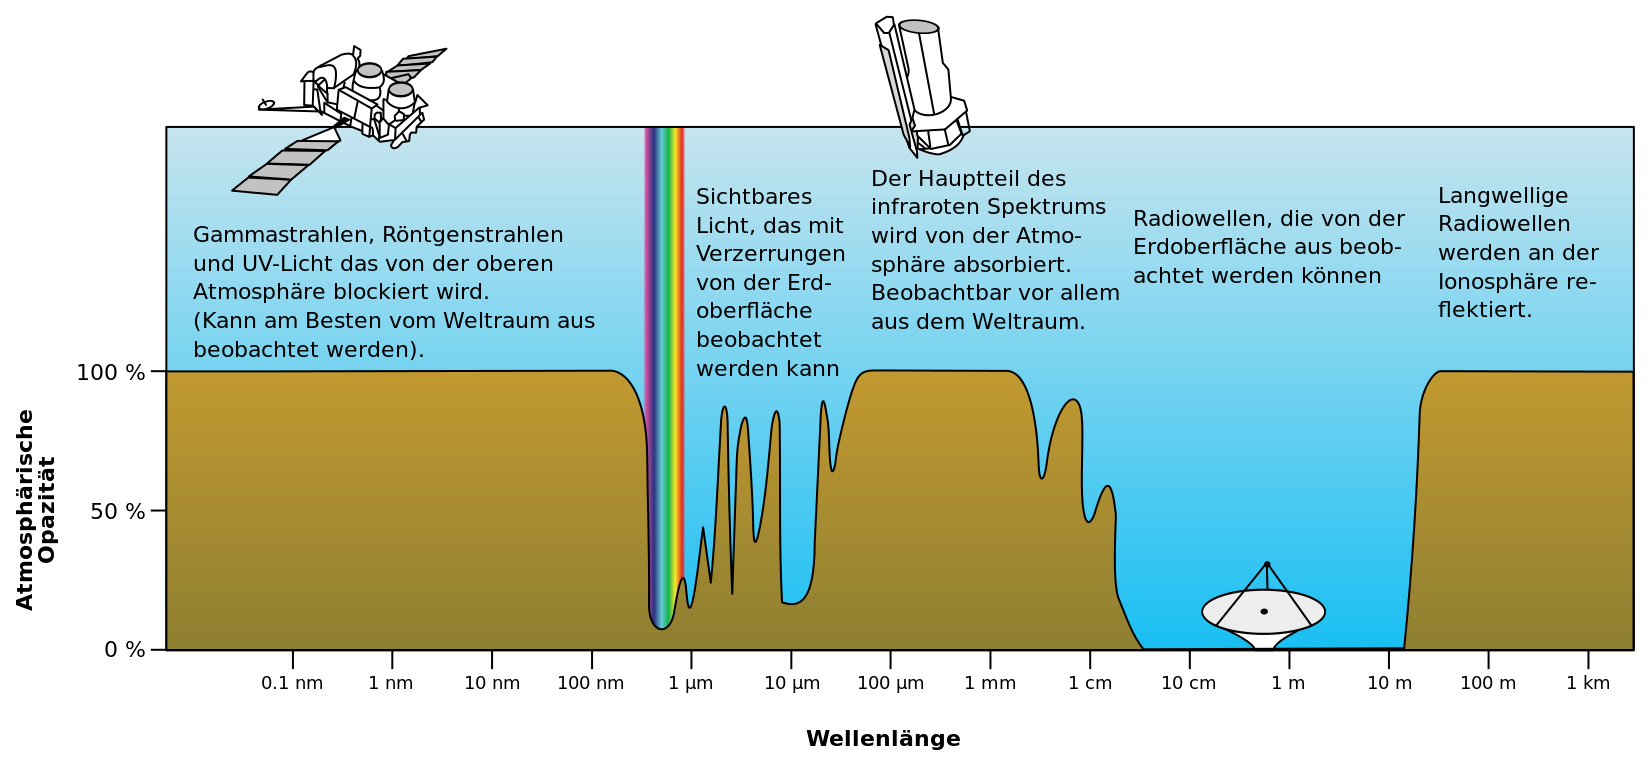
\includegraphics[width=0.9\textwidth]{images/Atmospheric.png}
  \end{figure}
\end{frame}
  \begin{frame}{Liegt es an der Zusammensetzung der Erdatmosphäre, dass nicht alle Frequenzen durchgelassen werden? Und wie kommt es, dass bestimmte Frequenzbereiche nicht durchgelassen werden?}
    \begin{columns}
   \begin{column}{0.4\textwidth}
    \begin{itemize}
      \item Ja es liegt an der Zusammensetzung der Atmosphäre
      \item Gase aborbieren bestimmte Wellenlängen
    \end{itemize}
  \vspace{2em}
  \end{column}
  \begin{column}{0.6\textwidth}
    \begin{figure}
      \centering
      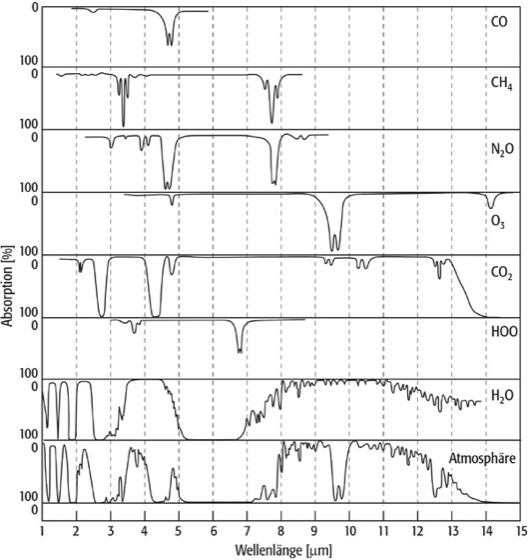
\includegraphics[width=0.65\textwidth]{images/atmo_fen_w.jpg}
    \end{figure}
  \end{column}
    \end{columns}
  \end{frame}


\begin{frame}{}
  \textbf{Warum haben die Sonne / die Sterne ein Schwarzkörperspektrum?}
  \begin{itemize}
    \item Schwarzer Strahler: reflektiert kein Licht, sendet Wärmestrahlung aus die nur von der Oberfläche und Temperatur abhänig ist
    \item Sonne ist auch ein Wärmestrahler
  \end{itemize}
  \textbf{Was sind Feld-Quanten?}
  \begin{itemize}
    \item Eichbosonen / Austauschteilchen
    \item Photonen, Gluonen, $Z^0$, $Z^\pm$
  \end{itemize}
  \textbf{Wofür ist die Friedmann-Gleichung}
  \begin{itemize}
    \item Beschreibung der Entwicklung des Universums
    \end{itemize}
\end{frame}

\begin{frame}{Wodurch genau ist die Rotverschiebung charakterisiert?}
  \begin{columns}
 \begin{column}{0.5\textwidth}
  \begin{itemize}
    \item Kosmische Rotverschiebung aufgrund der Ausdehnung des Universums
    \item Rotverschiebung aufgrund des Dopplereffektes: Bewegung, z.B. bei Spiralgalaxien
  \end{itemize}
  \end{column}
\begin{column}{0.5\textwidth}
  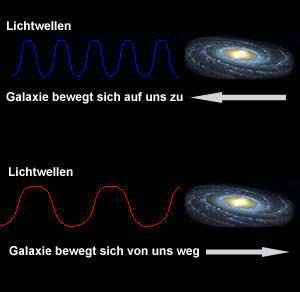
\includegraphics[width=\textwidth]{images/doppler.jpg}
\end{column}
  \end{columns}
\end{frame}

\begin{frame}{Was genau ist das Wasserstoffbrennen und wodurch entsteht es? Wie genau funktioniert der Energietransport bei Sternen? Was genau ist das Eddington-Limit?   Wie sieht der Lebeneslauf eines Sternes aus?
Aus welchen Elementen bestehen die meisten Sterne?  Was sind typische Ursachen für Dichtefluktuationen, die zur Entstehung neuer Sterne führt? Warum leben leichte Sterne länger als schwere?}
\end{frame}

\begin{frame}{Worin liegt genau der Unterschied zwischen einer Supernovae Typ I und Supernovae Typ II?
Was genau ist eine Wind-Supernovae und warum hat sie einen anderen Fluss als die SN-ISM? Wofür steht ISM?}
\end{frame}

\begin{frame}{Wie kommt es zur variablen Helligkeit der Cepheiden?}
\end{frame}

\begin{frame}{Was genau ist das Hubbelgesetz und die Hubbelkonstante und wofür ist es?}
\end{frame}
